\documentclass[aspectratio=1610,11pt]{beamer}

% Package to include videos
%\usepackage{multimedia}
\usepackage{animate}


% Use latex font theme in math mode
\usepackage[T1]{fontenc}
\usepackage{lmodern}
%\usefonttheme[onlymath]{serif}
\usefonttheme{professionalfonts}
%\usefonttheme[]{default}

\setbeameroption{hide notes} % Only slides
%\setbeameroption{show only notes} % Only notes
%\setbeameroption{show notes on second screen=right} % Both

%Load theme
\usetheme{KTH}
% remove this if using XeLaTeX or LuaLaTeX
%\usepackage[utf8]{inputenc}

% Multirow tables
\usepackage{multirow}

% So pgfplot doesnt complain (overleaf)
%\pgfplotsset{compat=1.18}

% To draw a grid on top of your images
\usetikzlibrary{calc}

% Animate list of images with zero pad for numbering
\makeatletter
\let\zeropad\@anim@pad
\makeatother

% Uncomment this if you want the table of contents to pop up at the 
% beginning of each section (you can do the same with subsections):
%\AtBeginSection[]
%{
%  \begin{frame}<beamer>{Outline}
%    \tableofcontents[currentsection]
%  \end{frame} \addtocounter{framenumber}{-1}
%}


\title[beamer stuff]{Using beamer}
\author{Josilio}
\date{\today}
\institute{KTH Mechanics}
\begin{document}


%%%%%%%%%%%%%%%%%%%%%%%%%%%%%%%%%%%%%%%%%%%%%%%%%%%%%%%%%%%%
\startpage
\begin{frame}[noframenumbering]

  \maketitle

\end{frame}


%%%%%%%%%%%%%%%%%%%%%%%%%%%%%%%%%%%%%%%%%%%%%%%%%%%%%%%%%%%%
\normalpageline


\begin{frame}{Overview}
\tableofcontents
\end{frame}

\section{General}
\subsection{Random stuff}
\begin{frame}[fragile]{\insertsection}
    \begin{itemize}
    \item You can \hl{highlight} text with \verb|\hl{}|. But I generally save the highlighting for \verb|\texttt{}|
    \item You can also \verb|\alert{}| some \alert{text}
    \item If you want to use the \texttt{verbatim} or \texttt{listings} environment in beamer, you have to add the \texttt{fragile} option to the frame. But this could mess up some beamer features.
    \item If you have big images or videos, in \texttt{Overleaf} you can speed up the compilation by clicking the arrow next to \texttt{Recompile} and selecting the \texttt{Fast[draft]} option. 
    \item To compile without transitions add \texttt{handout} in your document class options.
    \item You can cite, for instance, THE BOOK: \cite{schmid2002stability}

    \item I don't really like footnotes\footnotemark[1]
    
    \end{itemize}
    \footnotetext[1]{but sometimes they can help}
\end{frame}

\subsection{Transitions}
\begin{frame}[fragile]{\insertsection}
    \begin{itemize}
        \item Here are some commands for transitions
        \begin{itemize}
            \item \verb|\pause|
            \item \verb!\only<1|handout:0>{}!
            \item \verb!\onslide<2-|handout:2>{}!
        \end{itemize}
        \item For environments you can use, for instance,
         \begin{lstlisting}[language=tcl,numbers=none]
\item<1-> Some item\end{lstlisting}
         \begin{lstlisting}[language=tcl,numbers=none]
\alert<1>{text}  \textcolor<2>{color}{text}  \textbf<2>{text}\end{lstlisting}
         \begin{lstlisting}[language=tcl,numbers=none]
\begin{block}{}<3->
A block
\end{block}\end{lstlisting}
    \end{itemize}
        
\end{frame}

\subsection{Blocks}
\begin{frame}{\insertsection}{\insertsubsection}  
    \begin{block}{Normal block}
    And its body
    $$ \Reyn= 1e6$$
    Let's pause 
    \end{block}
    \pause
    \begin{exampleblock}{Example block}
    And its body
    \end{exampleblock}
    \begin{alertblock}{Alert block}<3->
    And its body
    \end{alertblock}
\end{frame}






\section{Colors and symbols}
\begin{frame}{\insertsection}
    \begin{columns}[t]
        \begin{column}{0.33\textwidth}
            \underline{KTH colors}
            \begin{itemize}
                \item \textcolor{kthcolor}{kthcolor}
                \item \textcolor{kthcolor_light}{kthcolor\_light}
                \item \textcolor{kthcolor_green}{kthcolor\_green}
                \item \textcolor{kthcolor_pink}{kthcolor\_pink}
                \item \textcolor{kthcolor_gray}{kthcolor\_gray}
            \end{itemize}
        \end{column}
        \begin{column}{0.33\textwidth}
            \underline{Matlab colors}
            \begin{itemize}
                \item \textcolor{matlabcolor1}{matlabcolor1}
                \item \textcolor{matlabcolor2}{matlabcolor2}
                \item \textcolor{matlabcolor3}{matlabcolor3}
                \item \textcolor{matlabcolor4}{matlabcolor4}
                \item \textcolor{matlabcolor5}{matlabcolor5}
                \item \textcolor{matlabcolor6}{matlabcolor6}
                \item \textcolor{matlabcolor7}{matlabcolor7}
            \end{itemize}
        \end{column}
        \begin{column}{0.33\textwidth}
            \underline{Python colors}
            \begin{itemize}
            \item \textcolor{tab_blue}{tab\_blue}
            \item \textcolor{tab_orange}{tab\_orange}
            \item \textcolor{tab_green}{tab\_green}
            \item \textcolor{tab_red}{tab\_red}
            \item \textcolor{tab_purple}{tab\_purple}
            \item \textcolor{tab_brown}{tab\_brown}
            \item \textcolor{tab_pink}{tab\_pink}
            \item \textcolor{tab_gray}{tab\_gray}
            \item \textcolor{tab_olive}{tab\_olive}
            \item \textcolor{tab_cyan}{tab\_cyan}
            \end{itemize}
        \end{column}
    \end{columns}
\end{frame}





\begin{frame}{\insertsection}
These two packages have icons and symbols that can be used as text. In the links you can find a complete list.
\begin{columns}[t]
    \begin{column}{0.5\textwidth}
       Font Awesome \href{https://mirrors.ibiblio.org/CTAN/fonts/fontawesome/doc/fontawesome.pdf}{[Link]}
       \begin{itemize}
           \item \faHeart
           \item \textcolor{kthcolor}{\faThumbsOUp}
           \item \textcolor{kthcolor_green}{\faLeaf} \faLeaf
           \item \textcolor{kthcolor_pink}{\faBicycle}
           \item \faInstagram
       \end{itemize}
    \end{column}
    \begin{column}{0.5\textwidth}
       manfnt \href{https://ctan.org/pkg/manfnt}{[Link]}
       \begin{itemize}
           \item \manconcentriccircles
           \item \textcolor{matlabcolor3}{\manstar} \manstar
           \item \mancube
       \end{itemize}
    \end{column}
\end{columns}
\end{frame}


\section{Adding videos}
\begin{frame}[fragile]{\insertsection}
    \begin{itemize}
        \item Load the package:  (see \href{http://ctan.unsw.edu.au/macros/latex/contrib/animate/animate.pdf}{documentation})
        \begin{lstlisting}[language=tcl,numbers=none]
\usepackage{animate} \end{lstlisting}
        \item One needs a bunch of images (not the video). 
        \item The pdf gets quite big and remember there is a  max limit of files in \texttt{Overleaf}.
        \item For zero padding, one can add the following: (see \href{https://tex.stackexchange.com/questions/86632/how-to-deal-with-zero-padding-using-multiframe-in-the-animate-package}{stackexchange post})
        \begin{lstlisting}[language=tcl,numbers=none]
\makeatletter
\let\zeropad\@anim@pad
\makeatother\end{lstlisting}
        \item For me, the visualisation has only worked on \texttt{Adobe Reader}. It also works on \texttt{Okular}, but not always in \texttt{Presentation mode}. Using \texttt{Full Screen Mode} should work okay; just missing the annotation tools available in \texttt{Presentation Mode}. Remember to tick the \texttt{Show form} box (> Edit)
    \end{itemize}
\end{frame}


\begin{frame}{\insertsection}
    \begin{animateinline}[poster=last,autoplay,autopause,loop,controls]{20}
    \multiframe{20}{i=0+1}{
\includegraphics[width=\textwidth]{impulse_images/impWv2\zeropad{0000}{\i} }
    }
    \end{animateinline}
\end{frame}



\section{Frames backgrounds}
\darkpageline
\begin{frame}[fragile]{\insertsection}
\begin{columns}
\begin{column}{0.5\textwidth}
    \begin{itemize}
        \item We can have a dark background using: 
        \begin{lstlisting}[language=tcl,numbers=none]
\darkpageline\end{lstlisting}
        \item There is even a 
        \begin{lstlisting}[language=tcl,numbers=none]
\startpagedark\end{lstlisting}
    \item Code looks cool:
        \begin{lstlisting}[language=Python]
import numpy as np
a = 3 #comment
for i in range(a):
    print(i)\end{lstlisting}
    \end{itemize}
    \end{column}

\begin{column}{0.5\textwidth}
    \begin{block}{Normal block}
    And its body
    \end{block}
    \begin{exampleblock}{Example block}
    And its body
    \end{exampleblock}
    \begin{alertblock}{Alert block}
    And its body
    \end{alertblock}
    \begin{equation}
        c^2 = a^2 + b^2
    \end{equation}
    \end{column}
    \end{columns}
\end{frame}
\startpagedark
\begin{frame}
    \maketitle
\end{frame}





\darkpageline
\begin{frame}{\insertsection}
    Images with transparent background look cool too
    \begin{animateinline}[poster=last,autoplay,autopause,loop]{15}
    \multiframe{20}{i=0+1}{
\includegraphics[width=\textwidth]{impulse_images/impWv2\zeropad{0000}{\i} }
    }
    \end{animateinline}
\end{frame}



\normalpageline
\begin{frame}[fragile]{\insertsection}
    \begin{itemize}
        \item We can go back to a normal page by: 
        \begin{lstlisting}[language=tcl,numbers=none]
\normalpageline\end{lstlisting}
    \end{itemize}
\end{frame}



\normalpagewaves
\begin{frame}[fragile]{\insertsection}
    \begin{itemize}
        \item Or using:
        \begin{lstlisting}[language=tcl,numbers=none]
\normalpagewaves\end{lstlisting}
        If you want some waves at the bottom 
    \end{itemize}
\end{frame}



\whitepage
\begin{frame}[fragile]{\insertsection}
    \begin{itemize}
        \item Or a totally blank page:
        \begin{lstlisting}[language=tcl,numbers=none]
\whitepage\end{lstlisting}
    \end{itemize}
\end{frame}

\darkpage
\begin{frame}[fragile]{\insertsection}
    \begin{itemize}
        \item Or a totally dark page:
        \begin{lstlisting}[language=tcl,numbers=none]
\darkpage\end{lstlisting}
    \end{itemize}
\end{frame}


\normalpageline
\section{TIKZ it!}
\begin{frame}[fragile]{\insertsection}
\begin{columns}
\begin{column}{0.5\textwidth}
\begin{itemize}
    \item Generate a grid on top of your image so you can see the local coordinates
    \item You have to add :
        \begin{lstlisting}[language=tcl,numbers=none]
 \usetikzlibrary{calc}\end{lstlisting}
    \item Once you are done drawing, you just have to comment the grid and axis labels
\end{itemize}
\end{column}
\begin{column}{0.5\textwidth}
    
     \begin{tikzpicture}
            %% Include the image in a node
            \node [
                above right,
                inner sep = 0,opacity=1,] (image) at (0,0) {
\includegraphics[width=0.8\textwidth]{kthgraphics/KTH-logo.pdf}};
            %% Create scope with normalized axes
            \begin{scope}[
                x={($0.1*(image.south east)$)},
                y={($0.1*(image.north west)$)}]
            %% Grid
                \draw[lightgray,step=1] (image.south west) grid (image.north east);
            %% Axes' labels
                \foreach \x in {0,1,...,10} { \node [below] at (\x,0) {\x}; }
                \foreach \y in {0,1,...,10} { \node [left] at (0,\y) {\y};}
            %% Your drawings
                \node[rotate=-90] at (8,8) {\textcolor{kthcolor_pink}{\faHeart}};
                \draw[kthcolor_green, very thick] (1,0.5) -- (9,1);
                \draw[kthcolor_light, very thick] (1.5,1.5) rectangle (8.5,8.5);
            \end{scope}
            \end{tikzpicture}
            \end{column}
            \end{columns}
\end{frame}


\begin{frame}[t]{Frame coordinate system}
	{Absolute positioning of images and sketches}
	%
	% Coordinate system for the page:
	%
	% -------------------------
	% |(0,1)             (1,1)|
	% |                       |
	% |       (0.5,0.5)       |
	% |                       |
	% |(0,0)             (1,0)|
	% -------------------------
	%
	% invoke by:
	% \node[nodeOptions] (nodeName) at (page cs:xNode,yNode) {nodeContents};

	\begin{tikzpicture}[remember picture,overlay]
		\node (sw) at (page cs:0,0) {+}; % bottom left
		\node (se) at (page cs:1,0) {+}; % bottom right
		\node (ne) at (page cs:1,1) {+}; % top    right
		\node (nw) at (page cs:0,1) {+}; % top    left

		\draw (sw) -- (se) -- (ne) -- (nw) -- cycle; % outer rectangle
		\draw (sw) -- (ne); % diagonals
		\draw (se) -- (nw); % diagonals
		%\draw[red,thick] (sw) -- (se);
		%\draw[green,thick] (se) -- (ne);

		\node (ce) at (page cs:0.5,0.5) {+}; % center

		\node (image) at (page cs:0.75,0.75) {% 
			
\includegraphics[width=.105\paperwidth]{kthgraphics/KTH-logo.pdf}%
		};
		\node (image) at (page cs:0.15,0.85) {% 
			
\includegraphics[width=.105\paperwidth]{kthgraphics/KTH-logo.pdf}%
		};
	\end{tikzpicture}
    
\end{frame}


\darkpageline
\begin{frame}{\insertsection}{pgfplots}
    \begin{columns}
        \begin{column}{0.5\textwidth}
            \resizebox{\textwidth}{!}{%
            \begin{tikzpicture}
                \begin{axis}[
                    title=Plot from Equation,
                    xlabel = {$x$},
                    ylabel = {$f(x)$},
                    ]
                \addplot[color=matlabcolor1,
                    domain=-pi:pi, 
                    samples=100, ]{cos(deg(x))};
                \addplot[color=matlabcolor2,
                    domain=-pi:pi, 
                    samples=100, ]{sin(deg(x))};
                \end{axis}
            \end{tikzpicture}
            }%
        \end{column}
        \begin{column}{0.5\textwidth}
            \resizebox{\textwidth}{!}{%
            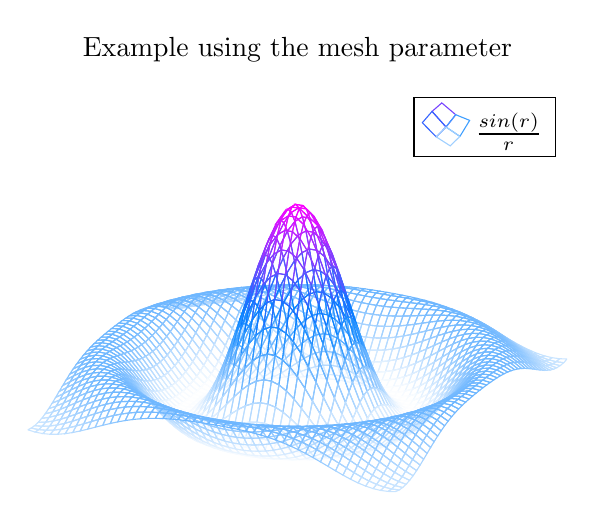
\begin{tikzpicture}
                \begin{axis}[
                    title=Example using the mesh parameter,
                    hide axis,
                    colormap/cool,
                    legend style={fill=none}
                    ]
                \addplot3[
                    mesh,
                    samples=50,
                    domain=-8:8,
                    ]
                    {sin(deg(sqrt(x^2+y^2)))/sqrt(x^2+y^2)};
                \addlegendentry{\(\frac{sin(r)}{r}\)}
                \end{axis}
            \end{tikzpicture}
            }%
        \end{column}     
    \end{columns}
\end{frame}


%% After this the pages are not counted anymore for the total number of slides
\appendix

\colorlet{darkBG}{NordDarkBlack} 
\darkpage
\begin{frame}
  \begin{tikzpicture}[remember picture,overlay]
		%\node () at (page cs:0.15,0.5) {
\includegraphics[width=.25\paperwidth]{kthgraphics/KTH-logo.pdf}};
		\node () at (page cs:0.15,0.5) {
\includegraphics[width=.25\paperwidth]{kthgraphics/KTH_Logotyp_RGB_2013_onlywhite.png}};
		\node () at (page cs:0.45,0.35) {
\includegraphics[width=.25\paperwidth]{logos/vinnova_logo.png}};
		\node () at (page cs:0.8,0.6) {
\includegraphics[width=.2\paperwidth]{logos/ERC_logo.png}};
		\node () at (page cs:0.45,0.6) {
\includegraphics[width=.25\paperwidth]{logos/naiss2.png}};
		\node () at (page cs:0.8,0.35) {
\includegraphics[width=.25\paperwidth]{logos/nffp.png}};
		\node () at (page cs:0.5,0.15) {\huge Thank you for your attention!};% 
		\node () at (page cs:0.5,0.08) {josfa@kth.se};% 
	\end{tikzpicture}

\end{frame}


\whitepage
 \begin{frame}[allowframebreaks]
 \frametitle{References}
 \bibliographystyle{apalike}
 \tiny{
\bibliography{references.bib}
}
\end{frame}

\end{document}
